\begin{section}{Problem 2}
    \begin{problem}{2}
        \begin{enumerate}[(a)]
            \item Download from the assignment webpage the file {\tt J\_GS.m}. In your {\sc Matlab} command line, run the command: {\tt J\_GS(100);} \\
            %\begin{verbatim}
            %J_GS(100); 
            %\end{verbatim}
            Include in your assignment solution the convergence graph that you are seeing. This is a linear system with the two-dimensional Laplacian of size $10,000 \times 10,000$ (we have $n=100, n^2=10,000$), and we are plotting the norm of the relative residual after 10,000 iterations for Jacobi and Gauss-Seidel. There is no reason to be impressed with this graph; convergence here is slow. But we are going to see  the effect of using SOR.
            \item Given the eigenvalues of the Laplacian in the slides, show that the optimal SOR parameter can be expressed as
            $$ \omega_{\rm opt} = \frac{2}{1+\sin \left( \frac{\pi}{n+1} \right)}.$$
            \item
            Modify the  {\sc Matlab} function so that in addition to the Jacobi and Gauss-Seidel graphs (for the same matrix) a convergence plot for the SOR method is included as well. Use the same initial guess (the zero vector) and the same stopping criterion: $\frac{\| \rr_k \|_2}{\| \bb \|_2} < 10^{-6}$. 
            
            {\underline {Tip}:} You should be seeing an {\em extremely dramatic} improvement in convergence. If you are not seeing such an improvement, then you must have done something wrong.
            \item Explain your results. 
        \end{enumerate}
    \end{problem}

    \newpage

    \begin{solution}{a}

        \textit{Note:} The line \begin{minted}{matlab}
            saveas(gcf, "DevamSisodraker_2a.jpg", "jpg");
        \end{minted} 
        was appended to the end of \textbf{{\tt J\_GS.m}} to ease the exporting process.
        \begin{mdframed}
            \footnotesize
            \textbf{File: {\tt J\_GS.m}}
            \inputminted{matlab}{J_GS.m}
            \normalfont
        \end{mdframed}

        \continued

        \begin{mdframed}
            \footnotesize
            \textbf{File: {\tt DevamSisodraker\_2a\_out.txt}}
            \inputminted{matlab}{DevamSisodraker_2a_out.txt}
            \normalfont
        \end{mdframed}

        \continued

        \begin{mdframed}[]
            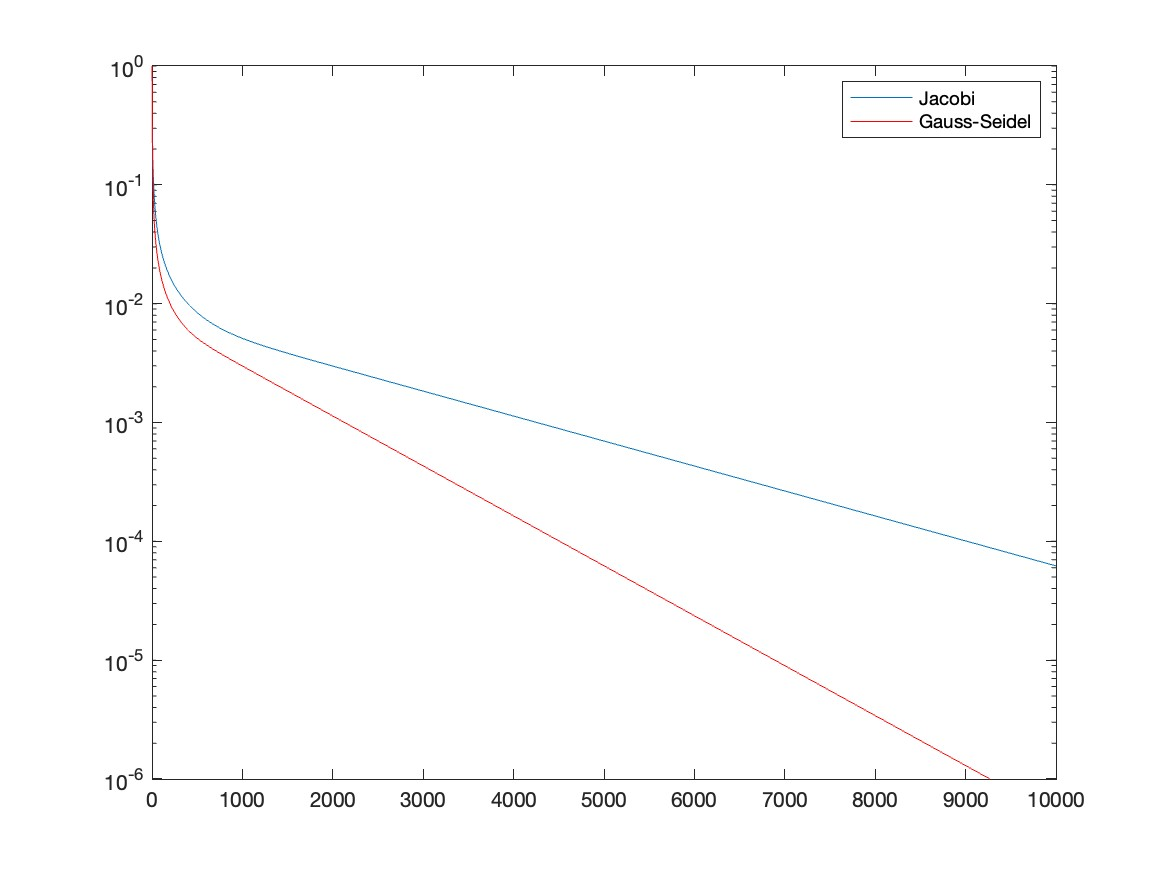
\includegraphics[scale=0.33]{DevamSisodraker_2a.jpg}
        \end{mdframed}

    \end{solution}

    \newpage
    
    \begin{solution}{b}
        The following is given in the lecture slides.
        \begin{align*}
            \lambda_{i,j} = 4 - 2 \left( \cos \frac{i \pi}{n + 1} + \cos \frac{j \pi}{n + 1} \right)
        \end{align*}
        Before we continue, let us first recall that the spectral radius of $T$ is given by $\mu_{1,1}$. Thus it follows that $\rho(T) = \mu_{i,i} = \cos \frac{\pi}{n + 1}$. Then let us substitute this $\rho(T)$ into the equation which defines $\omega_{opt}$.
        \begin{align*}
            \omega_{opt} &= \frac{2}{1 + \sqrt{1 - \left( \rho(T) \right)^2}} \\
            &= \frac{2}{1 + \sqrt{1 - \left( \cos \frac{\pi}{n + 1} \right)^2}} & \text{substitution of $\rho(T)$}\\
            &= \frac{2}{1 + \sqrt{\left( \sin \frac{\pi}{n + 1} \right)^2}} & \text{by Pythagorean trigonometric identity} \\
            &= \frac{2}{1 + \sin \frac{\pi}{n + 1}} & \\
        \end{align*}
    \end{solution}

    \newpage
    
    \begin{solution}{c}
        \begin{mdframed}
            \scriptsize
            \textbf{File: {\tt DevamSisodraker\_2c.m}}
            \inputminted{matlab}{DevamSisodraker_2c.m}
            \normalfont
        \end{mdframed}

        \continued

        \begin{mdframed}
            \footnotesize
            \textbf{File: {\tt DevamSisodraker\_2c\_out.txt}}
            \inputminted{matlab}{DevamSisodraker_2c_out.txt}
            \normalfont
        \end{mdframed}

        \continued

        \begin{mdframed}[]
            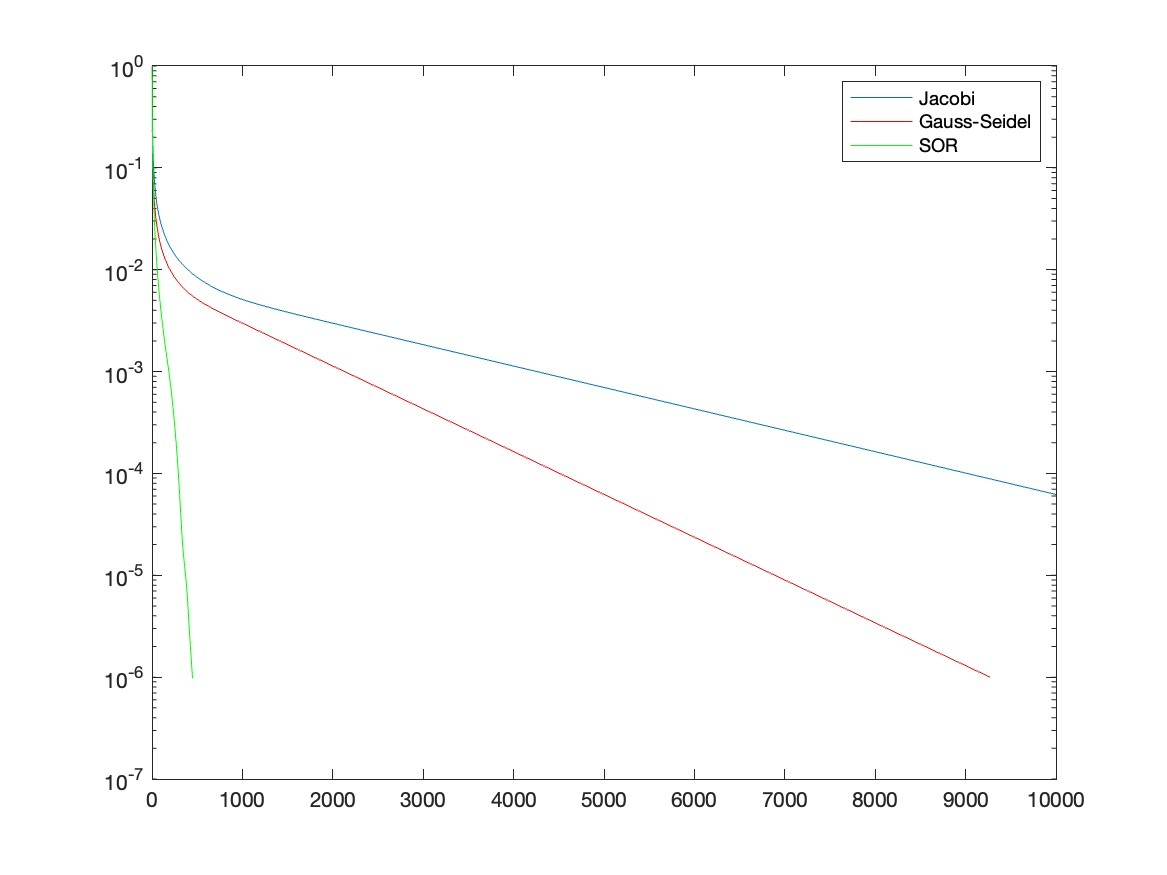
\includegraphics[scale=0.33]{DevamSisodraker_2c.jpg}
        \end{mdframed}
    \end{solution}

    \newpage
    
    \begin{solution}{d}
        \todo{write some bs explanation after you see a, b, c}
    \end{solution}

\end{section}